% Probably should just put diagrams and charts in data Visualization instead of here
% Just put accuracy and justification?
\section{Data Mining}\label{data_mining}

In this section, various data mining techniques are employed to extract meaningful insights from the preprocessed data.

\begin{description}[style=nextline]
    \item[Convolution Neural Network (CNN):] Detailed exposition of CNN model architecture and corresponding outcomes.
    \item[Multilayer Perceptron (MLP):] Elucidation of MLP model structure and ensuing results.
    \item[Comparison Between CNN and MLP:] Comparative analysis of CNN and MLP, along with justifications for the choice of each.
    \item[Supervised Machine Learning Algorithms:] Discussion on the non-utilization of supervised algorithms and reasons thereof.
    \item[Unsupervised Machine Learning Algorithms:] Explanation on the preference for CNN and MLP over unsupervised algorithms.
\end{description}

\subsection{Convolution Neural Network (CNN)}\label{cnn}

Convolutional Neural Networks (CNNs) are a powerful class of deep learning models that have achieved remarkable success in various image recognition and signal processing tasks. Their ability to automatically learn spatial features from the input data makes them particularly well-suited for analyzing sequential data like UWB CIR signals. In this work, a CNN is employed to classify the received UWB signals based on the location information they contain.

\subsubsection{Model Architecture}

The CNN model architecture comprises Conv1D, BatchNormalization, Dropout, Flatten, and Dense layers:

\begin{itemize}
    \item \textbf{Conv1D Layers:} Two Conv1D layers with 64 and 32 filters respectively, kernel size of 3, ReLU activation, and L2 regularization for preventing overfitting.
    \item \textbf{BatchNormalization Layers:} Normalize activations to accelerate training and reduce overfitting.
    \item \textbf{Dropout Layers:} Implemented with a rate of 0.5 to prevent overfitting by randomly dropping input units.
    \item \textbf{Flatten Layer:} Flattens the input for transitioning between convolutional and dense layers.
    \item \textbf{Dense Layers:} Two dense layers with 64 units and softmax activation for multi-class classification.
\end{itemize}

\subsubsection{Model Compilation and Training}

\begin{itemize}
    \item \textbf{Optimizer:} Adam optimizer with a learning rate of 0.0001.
    \item \textbf{Loss Function:} Categorical cross-entropy for multi-class classification.
    \item \textbf{Metrics:} Accuracy is chosen as the evaluation metric.
    \item \textbf{Early Stopping:} Training halts if validation loss doesn't improve for 10 consecutive epochs.
    \item \textbf{Training Parameters:} Trained for 20 epochs with a batch size of 32.
\end{itemize}


\subsubsection{Convolution Operation}

The core mathematical concept underlying the Conv1D layers is the convolution operation. In simpler terms, convolution can be understood through an analogy:

\begin{quote}
 Imagine a policeman investigating a crime scene. The policeman (filter) systematically scans the scene (input data) searching for evidence (features). By sliding a magnifying glass (kernel) across different areas, the policeman extracts crucial details (feature maps) that contribute to solving the crime (classification task).
\end{quote}

Mathematically, the convolution operation is defined as:

\begin{equation}
(f * g)(t) = \int_{-\infty}^{\infty} f(\tau)g(t - \tau) d\tau
\end{equation}

where:

\begin{itemize}
  \item $f$ and $g$ are the input data and the kernel, respectively
  \item $*$ denotes the convolution operation
  \item $t$ is the position at which the convolution is computed
  \item $\tau$ is the integration variable
\end{itemize}

In the context of CNNs, the integral is replaced by a summation over the discrete spatial dimensions (width in the case of Conv1D layers) of the input data and the kernel. The convolution operation essentially computes the dot product between the filter and the input data at each position, capturing the presence and strength of the specific feature the filter is designed to detect.

\subsubsection{Justification for not Pre-reducing Features}

One might consider explicitly extracting features from the UWB CIR signals before feeding them into the CNN. However, this approach has limitations. Handcrafted features might not capture the most relevant information for the classification task. In contrast, CNNs excel at automatically learning these features directly from the raw data during the training process. This allows the model to identify the most discriminative features for achieving optimal


% todo(ben): add info about how model is being trained %
\subsection{Multilayer Perceptron (MLP)}\label{mlp}                                                                                 
The Multilayer Perceptron (MLP) model is a class of feedforward artificial neural network that consists of at least three layers of nodes: an input layer, a hidden layer, and an output layer. MLPs are known for their ability to handle complex, non-linear relationships within the dataset, making them suitable for a wide range of classification tasks. Unlike simpler models, MLPs boast a layered structure with each layer fully connected to the next. This intricate architecture empowers them to unearth intricate patterns in the data and translate those patterns into accurate predictions. This capability is particularly valuable for NLOS/LOS classification, where signal characteristics can exhibit significant variations due to environmental factors.

\subsubsection{Model Architecture}

The MLP model used in this project was constructed using TensorFlow and Keras. The model architecture includes several Dense layers, BatchNormalization layers, and Dropout layers:

\begin{itemize}
    \item \textbf{Dense layers:} The model utilizes a sequential stack of Dense layers with ReLU activation for non-linearity. The first layer has 64 units, followed by layers with 32 and 16 units respectively. The final layer has a single unit with a sigmoid activation function suitable for binary classification (NLOS vs. LOS).
    \item \textbf{Regularization Techniques:} L2 regularization with a weight decay of 0.001 is applied to each Dense layer to penalize large weights and encourage smoother decision boundaries, reducing overfitting.
    \item \textbf{Normalization and Dropout:} BatchNormalization layers are inserted after each Dense layer to improve training speed and stability by normalizing activations. Dropout layers with a rate of 0.5 are strategically placed after BatchNormalization to randomly drop a fraction of activations during training, further preventing overfitting by encouraging the model to learn robust features that are not dependent on specific input units.
\end{itemize}

\subsubsection{Model Compilation and Training}

\begin{itemize}
    \item \textbf{Data Preparation:} Prior to training, data undergoes feature scaling using a StandardScaler object to ensure all features have a zero mean and unit variance. This improves the convergence of the optimization algorithm.
    \item \textbf{Train-Test Split:} The data is split into training and testing sets with an 80:20 ratio, ensuring a representative sample for model evaluation.
    \item \textbf{Early Stopping:} An EarlyStopping callback monitors the validation loss during training. Training is halted if the validation loss fails to improve for 10 consecutive epochs, preventing overfitting.
    \item \textbf{Model Compilation:} The model is compiled using the Adam optimizer with a learning rate of 0.0001 and binary cross-entropy loss function, suitable for binary classification tasks. Accuracy is chosen as the primary evaluation metric.
    \item \textbf{Training Process:} The model is trained for 20 epochs with a batch size of 32. The training history is captured to visualize the learning process later.
\end{itemize}

In this model, the ReLU (Rectified Linear Unit) activation function is used in the hidden layers, introducing a threshold for activation. The sigmoid function is used in the output layer, as it maps the output between 0 and 1, suitable for binary classification tasks (NLOS vs. LOS).

The MLP model utilizes the Adam optimization algorithm, which dynamically adjusts the weights and biases throughout the training process. Adam optimizes these parameters to minimize the binary cross-entropy loss function, which quantifies the disparity between the model's predictions and the actual labels. Minimizing this loss function enables the model to enhance its ability to accurately classify the input data, making it a crucial component of the training process.tra

% % Some figures from training %
\begin{figure}[H] 
	\centering
	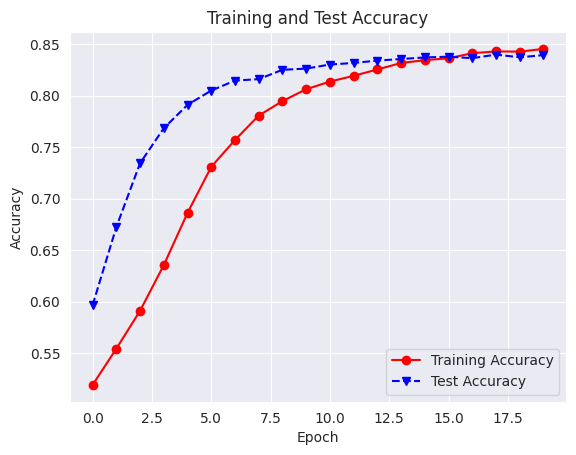
\includegraphics[width=0.50\textwidth]{mlp/Mlp_training_and_accuracy_plot}
	\caption{MLP training and test accuracy plot}\label{fig:mlp_training_and_accuracy_plot}
\end{figure}

A thorough analysis of the results reveals that the model maintains an accuracy of around 85\% throughout the epochs, indicating strong performance on the training data. In contrast, the test accuracy, though slightly lower than the training accuracy, remains stable around 80\% across epochs, suggesting reasonable generalization to unseen data. The observed gap between the training and test accuracy indicates potential overfitting, a common phenomenon where a model performs well on training data but struggles with unseen data.

\begin{figure}[H] 
	\centering
	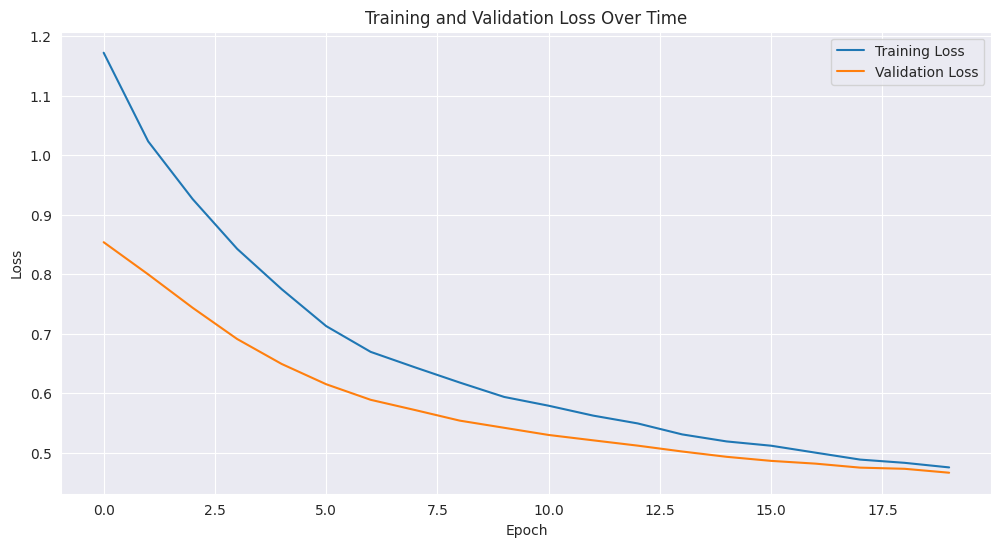
\includegraphics[width=0.50\textwidth]{mlp/Mlp_training_and_validation_loss_plot}
	\caption{MLP training and validation loss plot}\label{fig:mlp_training_and_validation_loss_plot}
\end{figure}

Additionally, the training and validation loss over time plot for this model shows a promising trend. It suggests that the model is learning effectively and avoiding overfitting. The training loss appears to be steadily decreasing over the epochs, indicating that the model is continually improving its ability to fit the training data. Similarly, the validation loss also shows a decreasing trend, although it fluctuates slightly more than the training loss. Overall, the validation loss follows a similar pattern to the training loss, indicating that the model is generalizing well and not overfitting to the training data.

\begin{figure}[H] 
	\centering
	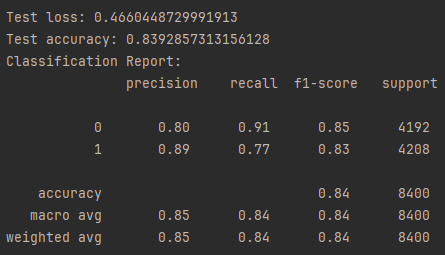
\includegraphics[width=0.50\textwidth]{mlp/Mlp_classification_report}
	\caption{Mlp training classification report}\label{fig:mlp_classification_report}
\end{figure}

% todo classification report Justification ^ %

\subsubsection{Multilayer Perceptron Operation}

The core mathematical concept underlying the Multilayer Perceptron (MLP) is the dot product operation, employed within the neurons of the Dense layers. In simpler terms, this can be understood through an analogy:

\begin{quote}
Imagine a robot deciding whether to go outside to play based on the weather. Each piece of information (input) about the temperature and weather condition (sunny or cloudy) is assigned a weight, representing its importance. The robot then calculates the total weighted sum of the inputs, adds a bias (its preference for certain weather conditions), and applies an activation function (decision rule) to determine if it should go outside (neuron activation).
\end{quote}

Mathematically, the output \(y\) of a single neuron is defined as:

\[
y = \phi \left( \sum_{i=1}^{n} w_i x_i + b \right)
\]

where:
\begin{itemize}
  \item \(w_i\) and \(x_i\) are the weights and input data, respectively
  \item \(n\) is the number of inputs to the neuron
  \item \(b\) is the bias
  \item \(\phi\) is the activation function
\end{itemize}

This operation essentially performs a weighted sum of the inputs, similar to linear regression. However, MLPs introduce non-linearity through activation functions, allowing them to learn more complex relationships between features and the output. This dot product operation can be visualized as a neuron taking a weighted sum of its input, adding a bias, and then passing the result through an activation function.

\subsection{Comparison Between CNN and MLP}\label{cnn_vs_mlp}

% Decide whether are you using supervised or unsupervised learning? What algorithm should be preferred for your team? %
% Decide the split ratio of the training/test dataset such as 70:30 or 80:20? %
% Determine the classification, regression performance accuracy such as RMSE, confusion matrix etc? %
\subsection{Supervised Machine Learning Algorithms}\label{sml}

% TO WRITE %


% Decide whether are you using supervised or unsupervised learning? What algorithm should be preferred for your team? %
% Decide the split ratio of the training/test dataset such as 70:30 or 80:20? %
% Determine the classification, regression performance accuracy such as RMSE, confusion matrix etc? %
\subsection{Unsupervised Machine Learning Algorithms}\label{uml}


% TO WRITE %
